\chapter{Coordinate Frames}
\label{sec:CoordianteFrames}

A very crucial part of this project, was the analysis of the MAV's coordinate systems. This is very important because the MAV takes its desired position from what it detects from its camera and has to transform it to the IMU frame with respect to the world frame. Furthermore, the apriltag's position in the simulated world is defined by it's pose as detected from the usb camera. For the transformations the ASL's minkindr library was used. It should be noted, that the color coding in the axes frames follows the RVIZ color convention, meaning blue defines the z axis, green the y axis and red the x axis respectively. Furthermore the ASL's frame naming convention \cite{FrameNamingConvention} is followed throughout this project. 

 \section{Coordinate Frames in the Simulation }
 \label{sec: CoordinatesinSimulation}
 
 The first thing that should be resolved in the simulation world, was the correct positioning of the apriltag with respect to the real camera detection. Although the two frames share the same origin point, the have different orientations as seen by figure \ref{pics:worldcamframe}, the distance between the two frames is set to emphasize the rotation. As it can easily be seen the transformation form camera frame to the world frame consists of one rotation of $90^{\circ}$ around the world's y axis $(rot_{y_{world}}(90^{\circ}))$ and a successive rotation of $-90^{\circ}$ around the current z axis $(rot_z(-90^{\circ}))$ as presented in the equation \ref{eq:camtoworldrot}. With the aforementioned transformation, the coordinates as seen from the camera match the actual world coordinates. Furthermore, it is easily understood that the apriltag's yaw in the real world corresponds to the negative pitch of the detected image.
 
 \begin{equation}
 \label{eq:camtoworldrot}
 \left[\begin{array}{c}
 x_{wc} \\ y_{wc} \\ z_{wc}  \end{array} \right] = Rot_{y_{world}}(90^{\circ})Rot_z(-90^{\circ})\left[ \begin{array}{c} x_c \\ y_c \\z_c \end{array} \right] = \begin{bmatrix} 0 & 0 & 1 \\ -1 & 0 & 0 \\ 0 & -1 & 0 \end{bmatrix} \left[ \begin{array}{c} x_c \\ y_c \\z_c \end{array} \right]
 \end{equation}
  
  
 \begin{figure}
    \centering
    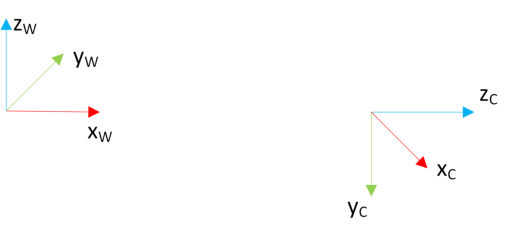
\includegraphics[width=0.98\textwidth]{images/world_camera_frame.pdf}
    \caption{The camera frame and the world frame.}
    \label{pics:worldcamframe}
 \end{figure}
 
 After the transformation of the camera frame, now come the coordinate transformations regarding the MAV. The Firefly's reference body frame coincides with its IMU frame. The real system sends the world's coordinates with respect to the aforementioned frame to the position controller so as to define its position. The camera frame as can be seen from the figure \ref{pics:mavcoordinateframe} is rotated and titled downwards relative to the IMU frame. The transformation between the inertial system and the MAV's body frame is provided by subscribing to the Firefly's odometry sensor, named as odometry\textunderscore sensor\textunderscore 1, the obtained transformation is represented by $T_{WB}$. Then, the transform from the body frame to the camera link frame is obtained, represented as $T_{BC}$. It should be noted, that since the aforementioned transform is static, it is pre-calculated and passed as a parameter to the system so speed up the procedure. So the final transformation from the camera to the world frame, noted as $T_{WC}$ is given by equation \ref{eq:TWC}. In order to simplify the hole process in simulation and since the error that is inserted is small, the coordinates of the camera with respect to the world are sent to the position controller.  
 
 \begin{equation}
 \label{eq:TWC}
 T_{WC} = T_{WB} * T_{BC}
 \end{equation}  
 
  \begin{figure}
     \centering
     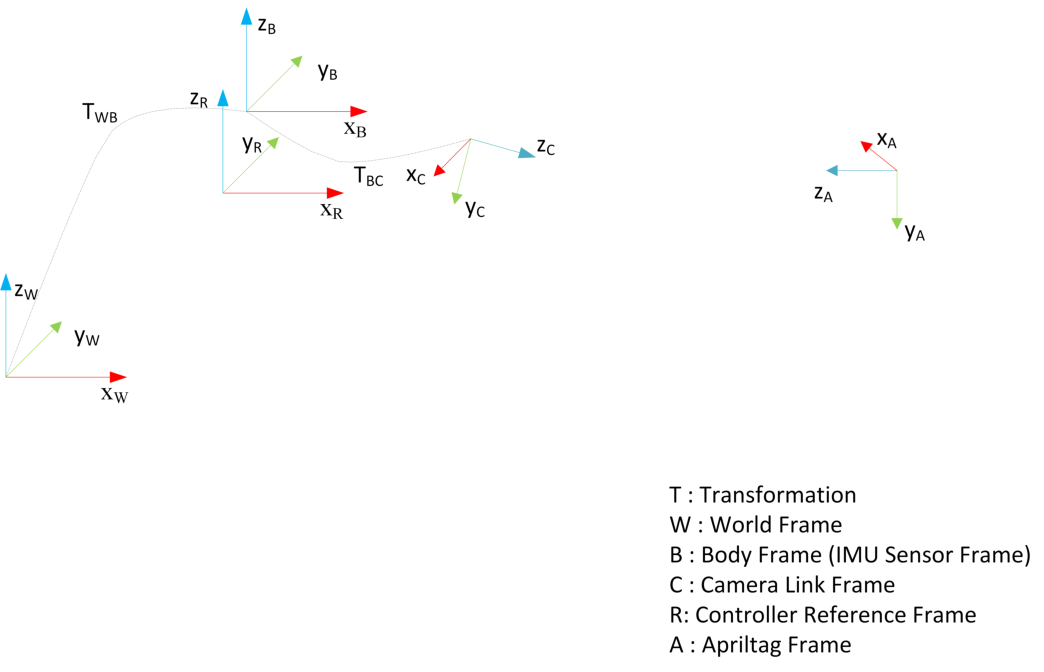
\includegraphics[width=0.98\textwidth]{images/coordinate_frame_representation_v2.pdf}
     \caption{The camera frame and the world frame.}
     \label{pics:mavcoordinateframe}
  \end{figure}
  
  
\section{Coordinate Frames in the Real System}
\label{sec: CoordinatesinRealSystem}
  